%=========================================================================
% (c) 2011, 2012 Josef Lusticky

\chapter{Measurements}\label{chap:measurements}
There are several factors that can be measured.
The clock interrupt frequency measurements show the influence of the clock adjustments
on the number of clock ticks (interrupts) per second.
The clock offset measurements show the time difference between the reference clock and
the local clock.
The clock phase measurements show the phase difference between the reference clock and
the local clock, that is, when each second is accounted.
All of the presented plots and their respective source values can be found on the CD
attached to this thesis.
The table of CD contents is listed in appendix~\ref{app:cd-contents}.
\begin{figure}[H]
	\centering
	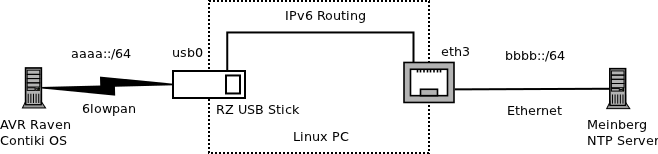
\includegraphics[width=13cm,keepaspectratio]{fig/radvd-routing.png}
	\caption{Network topology for measurements}
	\label{fig:measurements-routing}
\end{figure}
Figure~\ref{fig:measurements-routing} shows the network topology used for the measurements.
The reference clock for all of the presented measurements was
the Meinberg~M600 NTP stratum 1 server, which was synchronised using the GPS.
The NTP client was running on the AVR Raven platform in a room at 23~\textcelsius.

\section{Clock interrupt frequency}
The AVR Raven's bit 7 of Port D and the ground pin were
connected to the UNI-T~2025CEL digital oscilloscope
to measure the clock interrupt frequency.
At the beginning of the interrupt service routine a~logic 1 was written
to the bit 7 of Port D, what caused a high level of voltage.
At the end of the interrupt service routine a~logic 0 was written
to the bit 7 of Port D, what caused a low level of voltage.

When there are no clock adjustments in progress, the value of the output compare register is 31 by default.
The clock interrupt frequency
is supposed to be equal to the~value of the {\it{CLOCK\_SECOND}} macro, which is 128 by default on AVR~Raven
and is given by formula~\ref{equ:measurements-128}.
Figure~\ref{fig:app-osc-no-adjust} in appendix~\ref{app:interrupt-frequency} shows the oscilloscope output 
for this case.
\begin{equation}
\label{equ:measurements-128}
\frac{\frac{f_{asy}}{prescaler}}{counts} = \frac{\frac{32768}{8}}{32} = 128
\end{equation}

Figure~\ref{fig:app-osc-speed-up} in appendix~\ref{app:interrupt-frequency} shows the oscilloscope output
when slowing down the clock.
The clock interrupt frequency
is supposed to be equal to $124.\overline{12}$~Hz and is given by formula~\ref{equ:measurements-124}.
\begin{equation}
\label{equ:measurements-124}
\frac{\frac{f_{asy}}{prescaler}}{counts + 1} = \frac{\frac{32768}{8}}{32+1} = 124.\overline{12}
\end{equation}

Figure~\ref{fig:app-osc-slow-down} in appendix~\ref{app:interrupt-frequency} shows the oscilloscope output
when speeding up the clock.
The clock interrupt frequency
is supposed to be approximately equal to 132.129~Hz and is given by formula~\ref{equ:measurements-132}.
\begin{equation}
\label{equ:measurements-132}
\frac{\frac{f_{asy}}{prescaler}}{counts - 1} = \frac{\frac{32768}{8}}{32-1} \doteq 132.129
\end{equation}

The measured values are not exactly equal to those expected.
This is mostly because of a room temperature influence on the clock source
(32~768~Hz quartz crystal oscillator),
but it could also be air pressure or magnetic fields, etc.

\section{Clock offset}
\begin{figure}[H]
  \centering
  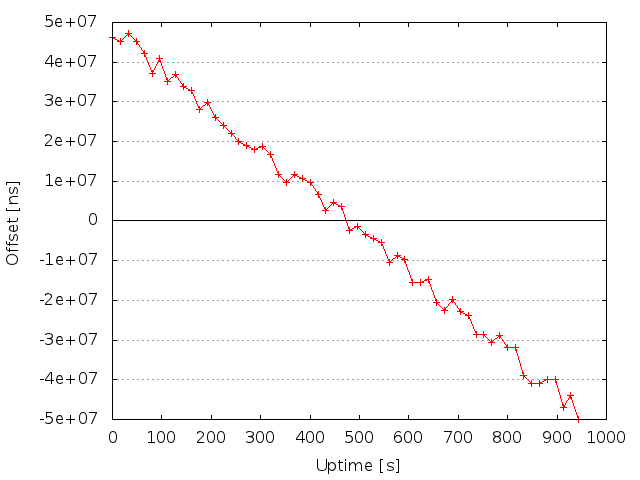
\includegraphics[width=11cm,keepaspectratio]{fig/no-ntp.png}
  \caption{Local clock offset without NTP client}
  \label{fig:measurements-no-ntp}
\end{figure}
Figure~\ref{fig:measurements-no-ntp} shows the local clock offset
in case no NTP client runs on the device.
The time is set with the initial offset of about 45 milliseconds.
However, the clock progresses faster because of frequency errors.
This compensates the initial clock offset at first,
but then it causes the offset increase.
The clock is running faster with approximately 100~PPM,
where 1~PPM is equal to $10^{-6}$ $\frac{s}{s}$ (0.0001\%).
That is, the clock error is about 9 seconds a day in this case.
The offset increase is not exactly linear because of the frequency jitter,
which can be also observed.

Figure~\ref{fig:measurements-ntp-serial} shows the local clock offset
acquired from the serial output in case the Contiki NTP client runs on the device.
When the developed NTP client receives a response from the server,
it calculates the local clock offset and prints its value to the serial output.
The NTP poll interval was set to 16 seconds, that means, the local clock offset
is calculated and eventually corrected every 16 seconds.
\begin{figure}[H]
  \centering
  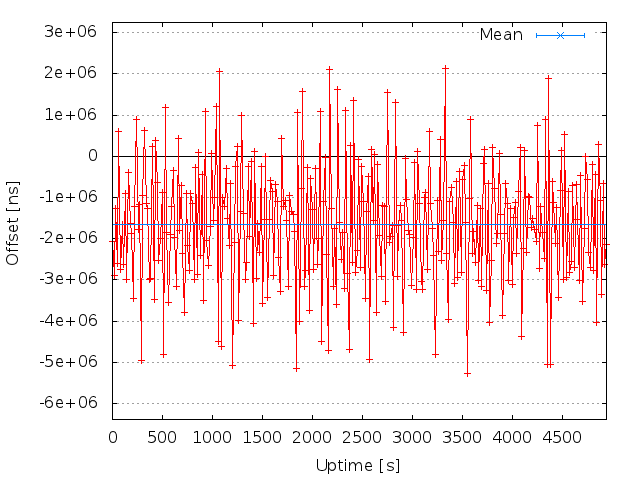
\includegraphics[width=11cm,keepaspectratio]{fig/poll-16s.png}
  \caption{Local clock offset with adjustments and NTP poll interval 16s}
  \label{fig:measurements-ntp-serial}
\end{figure}
The blue line shows the mean local clock offset value,
which should be equal to zero in a perfect case.
This is however not the case, because of the oscillator frequency error
shown in figure~\ref{fig:measurements-no-ntp}.
More figures showing the local clock offset measurements
can be found in appendix~\ref{app:offset}.

\section{Clock phase}
The GPS based clock Meinberg~GPS~167 and digital oscilloscope UNI-T~2025CEL
were used for measuring the clock phase difference.
Meinberg~GPS clock rises an impulse when each second is accounted.
Contiki on AVR~Raven was configured to write a logic~1
to~bit~7 of~Port~D when each second is accounted
and to write a logic~0 to~the same bit after~25 clock ticks.

When the NTP client uses the {\it{clock\_adjust\_time}} call,
the local clock offset as well as the phase is being adjusted.
Figure~\ref{fig:measurements-osc-adjusting-phase} shows the phase while adjusting the clock.
The yellow line is the output signal from Meinberg~GPS clock
and the blue line is the output signal from AVR~Raven.
\begin{figure}[H]
  \centering
  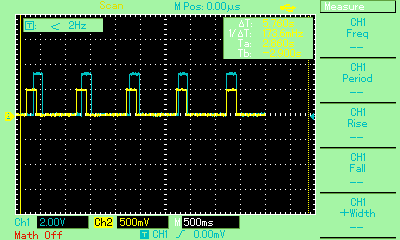
\includegraphics[width=11cm,keepaspectratio]{fig/osc-adjusting-phase.png}
  \caption{Second impulses when clock adjustments are in progress}
  \label{fig:measurements-osc-adjusting-phase}
\end{figure}
Figures showing the clock out of phase and in phase with
the reference clock can be found in appendix~\ref{app:phase}.
